\begin{minipage}{0.55\textwidth}
    \begin{figure}[h]
    \centering
    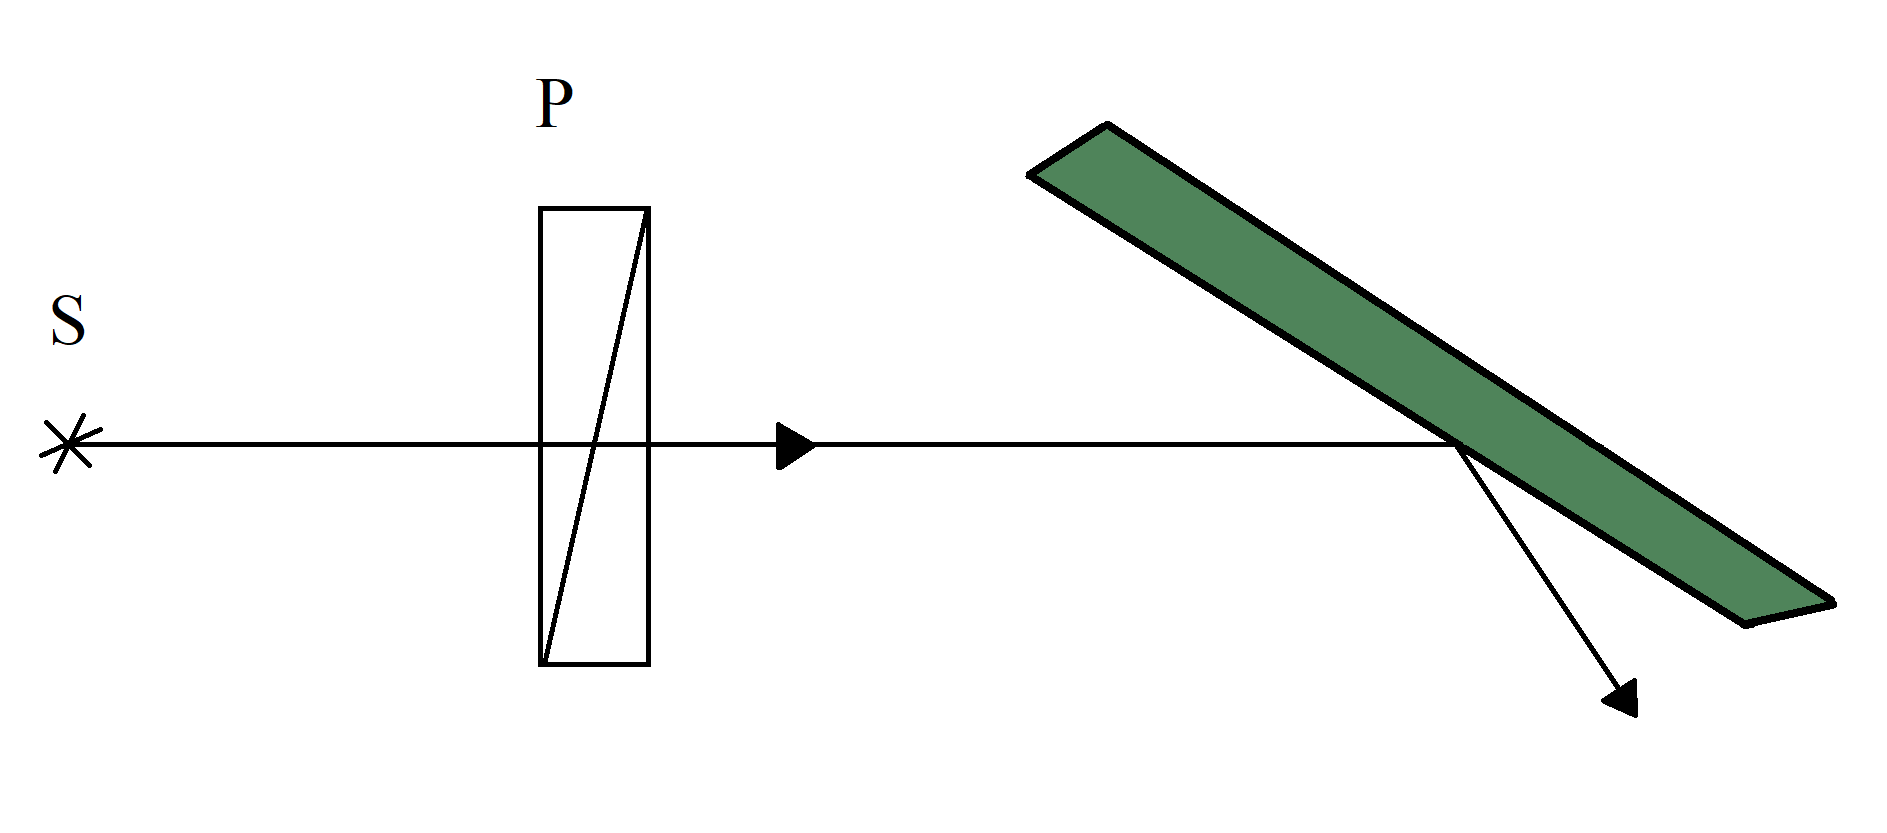
\includegraphics[width=1\textwidth]{images/ebonit.png}
    \caption{By rotating green ebonite plain we obtain several angles.}
    %\label{fig:}
\end{figure}
\end{minipage}
\hfill
\begin{minipage}{0.35\textwidth}
	\begin{center}
	\begin{tabular}{ |c|c|c| } 
		\hline
		name & $\theta_p$ & $\tg(\theta_p)$ \\
 		\hline
 		K & 240 & 1.73 \\ 
 		E & 237 & 1.54 \\ 
 		K & 237 & 1.54 \\ 
 		E & 238 & 1.60 \\ 
 		K & 236 & 1.48 \\ 
 		E & 239 & 1.66 \\ 
 		\hline
	\end{tabular}
	\end{center}
	The measurements were taken apart from each other.
\end{minipage}

